\subsection{SN-DCGAN}
\label{sec:exp-sndcgan}
We implement spectral normalization and use it on the discriminator of the DCGAN used in the previous section. We present the evolution of the Inception score and losses in Figures \ref{fig:exp-sndcgan-is} and \ref{fig:exp-sndcgan-losses}. We observe that both losses are much smoother with spectral normalization. This is the desired result; the original intent of the paper on spectral normalization was to provide a solution to stabilize the training of GANs \cite{miyato2018spectral}. By inspecting the generated images we observe a significant reduce in mode collapse and improvement of image quality. %This did however not result in a significant Inception score improvement.
\begin{figure}[H]
    \centering
    \begin{subfigure}[t]{0.49\textwidth}
        \centering
		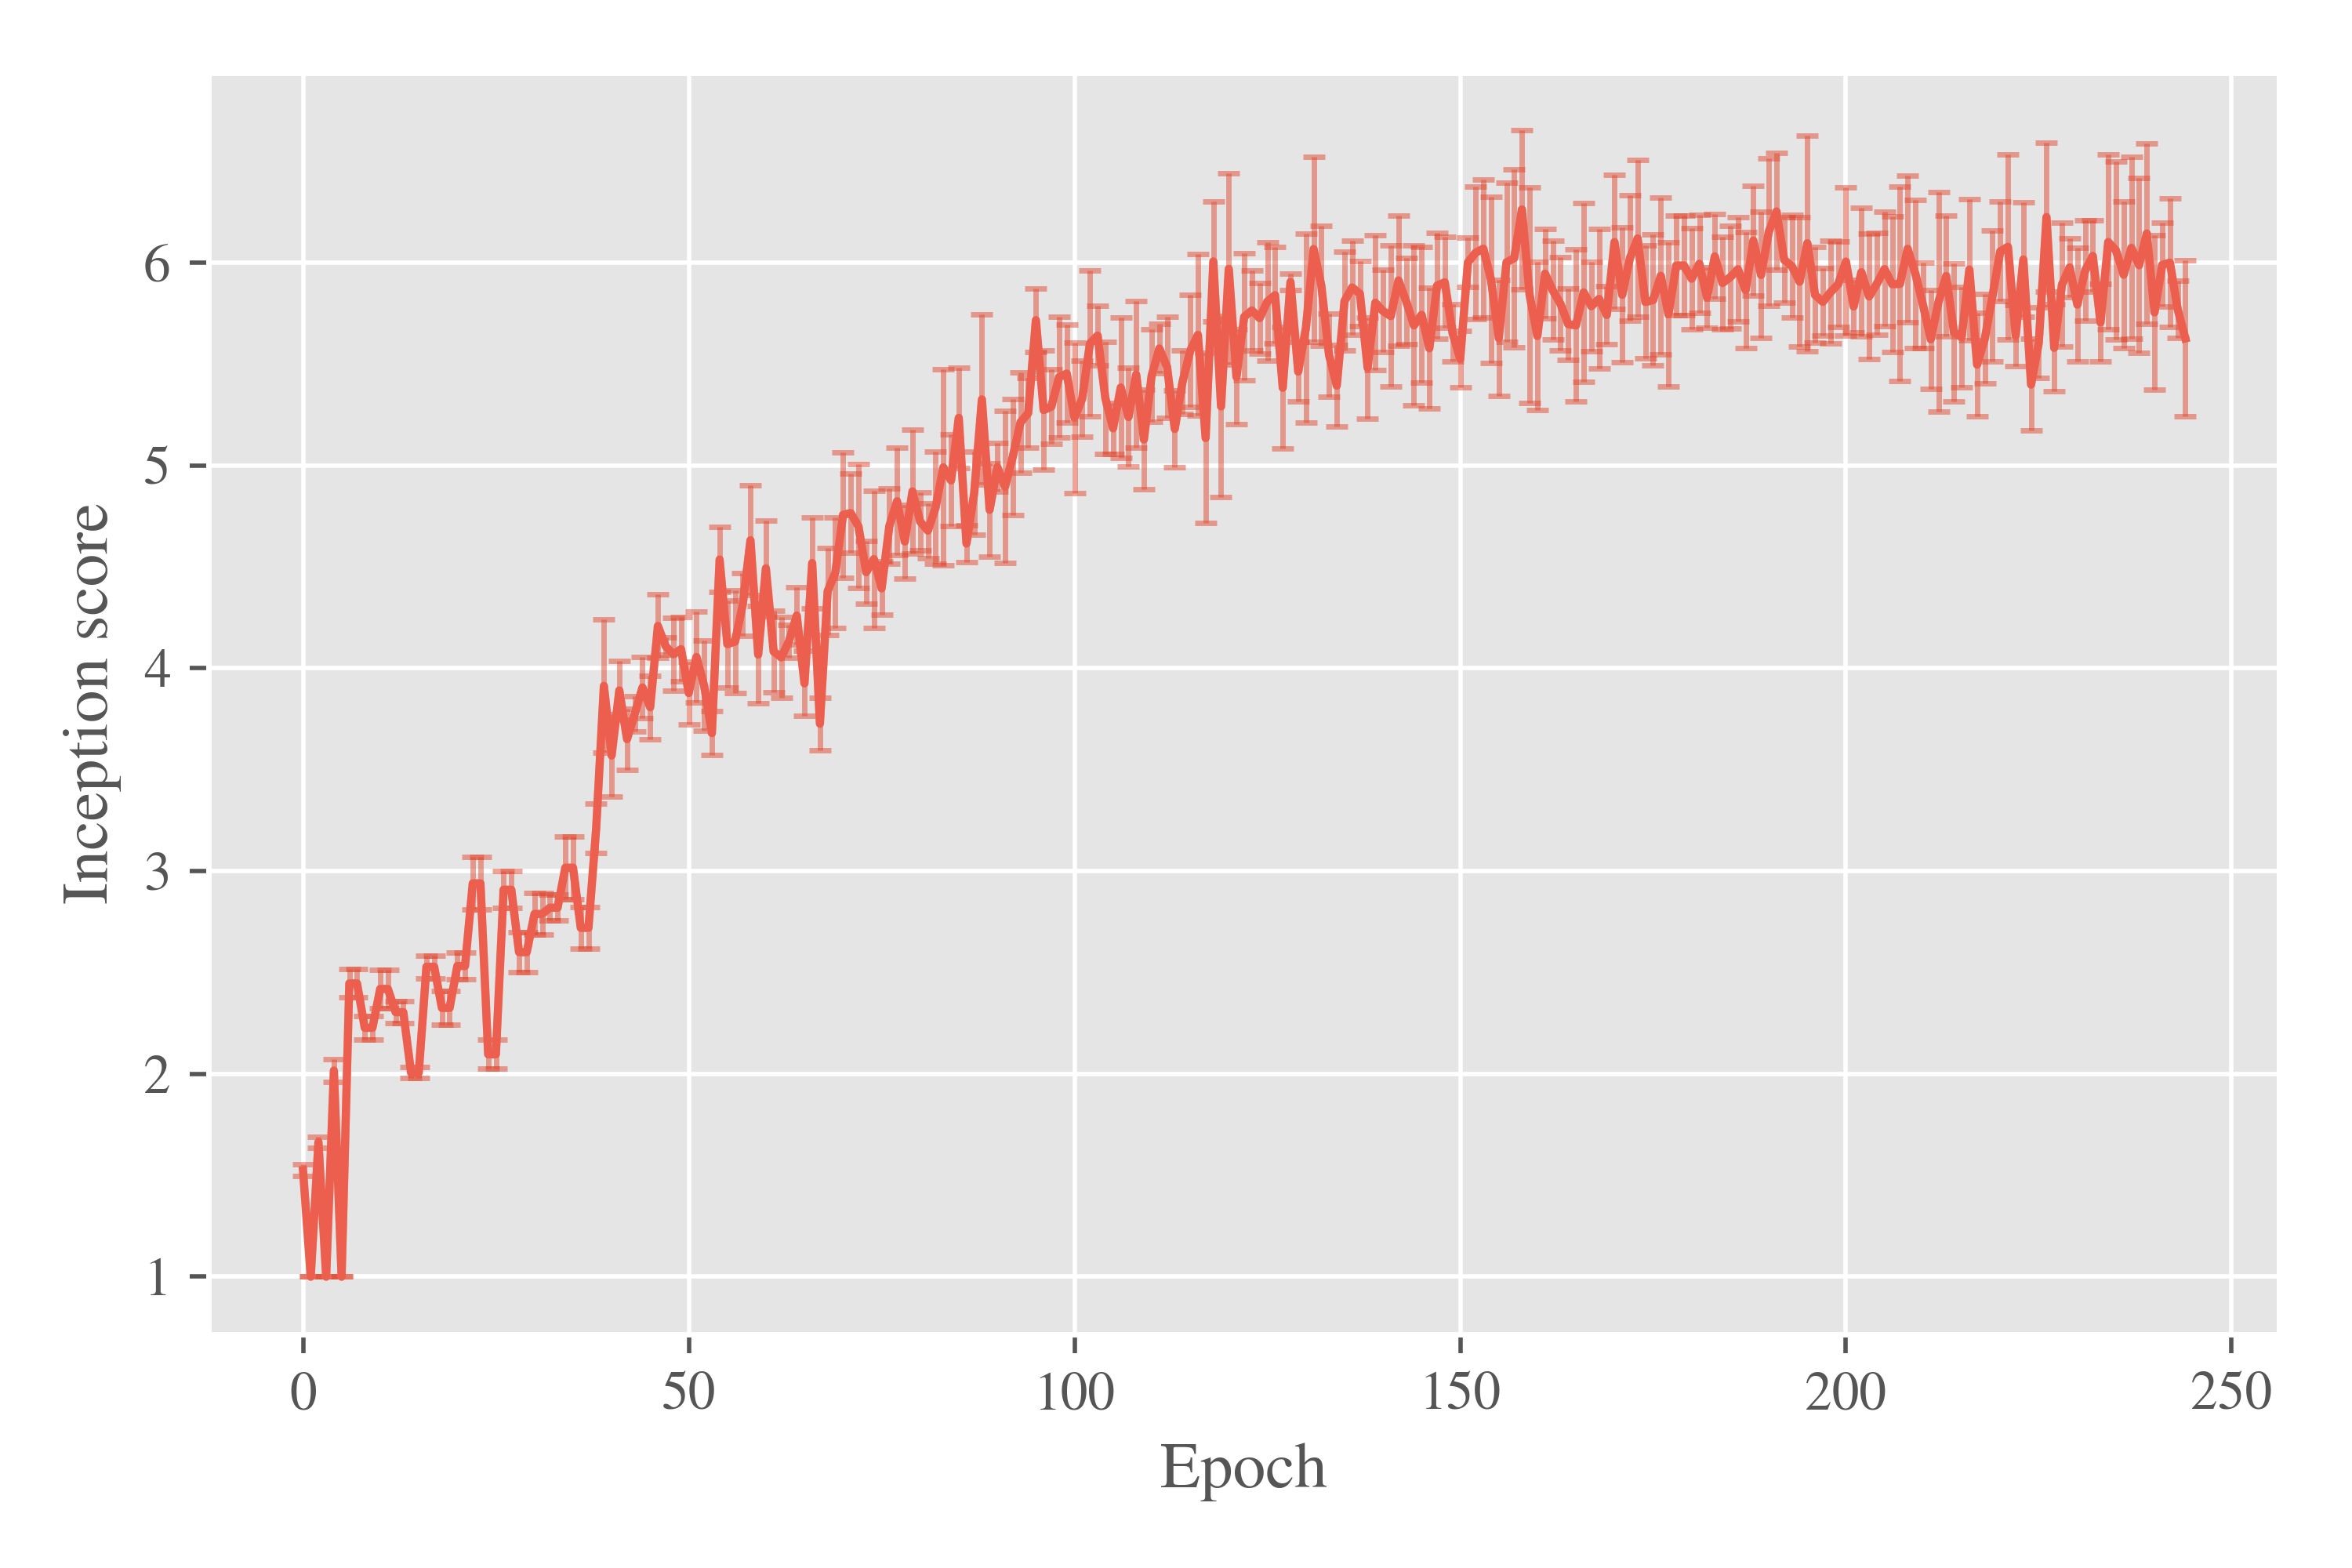
\includegraphics[width=\textwidth]{../code/results/figures/sndcgan_cifar10_is.png}
		\caption{Inception score\\~}
		\label{fig:exp-sndcgan-is}
    \end{subfigure}
    \begin{subfigure}[t]{0.49\textwidth}
        \centering
        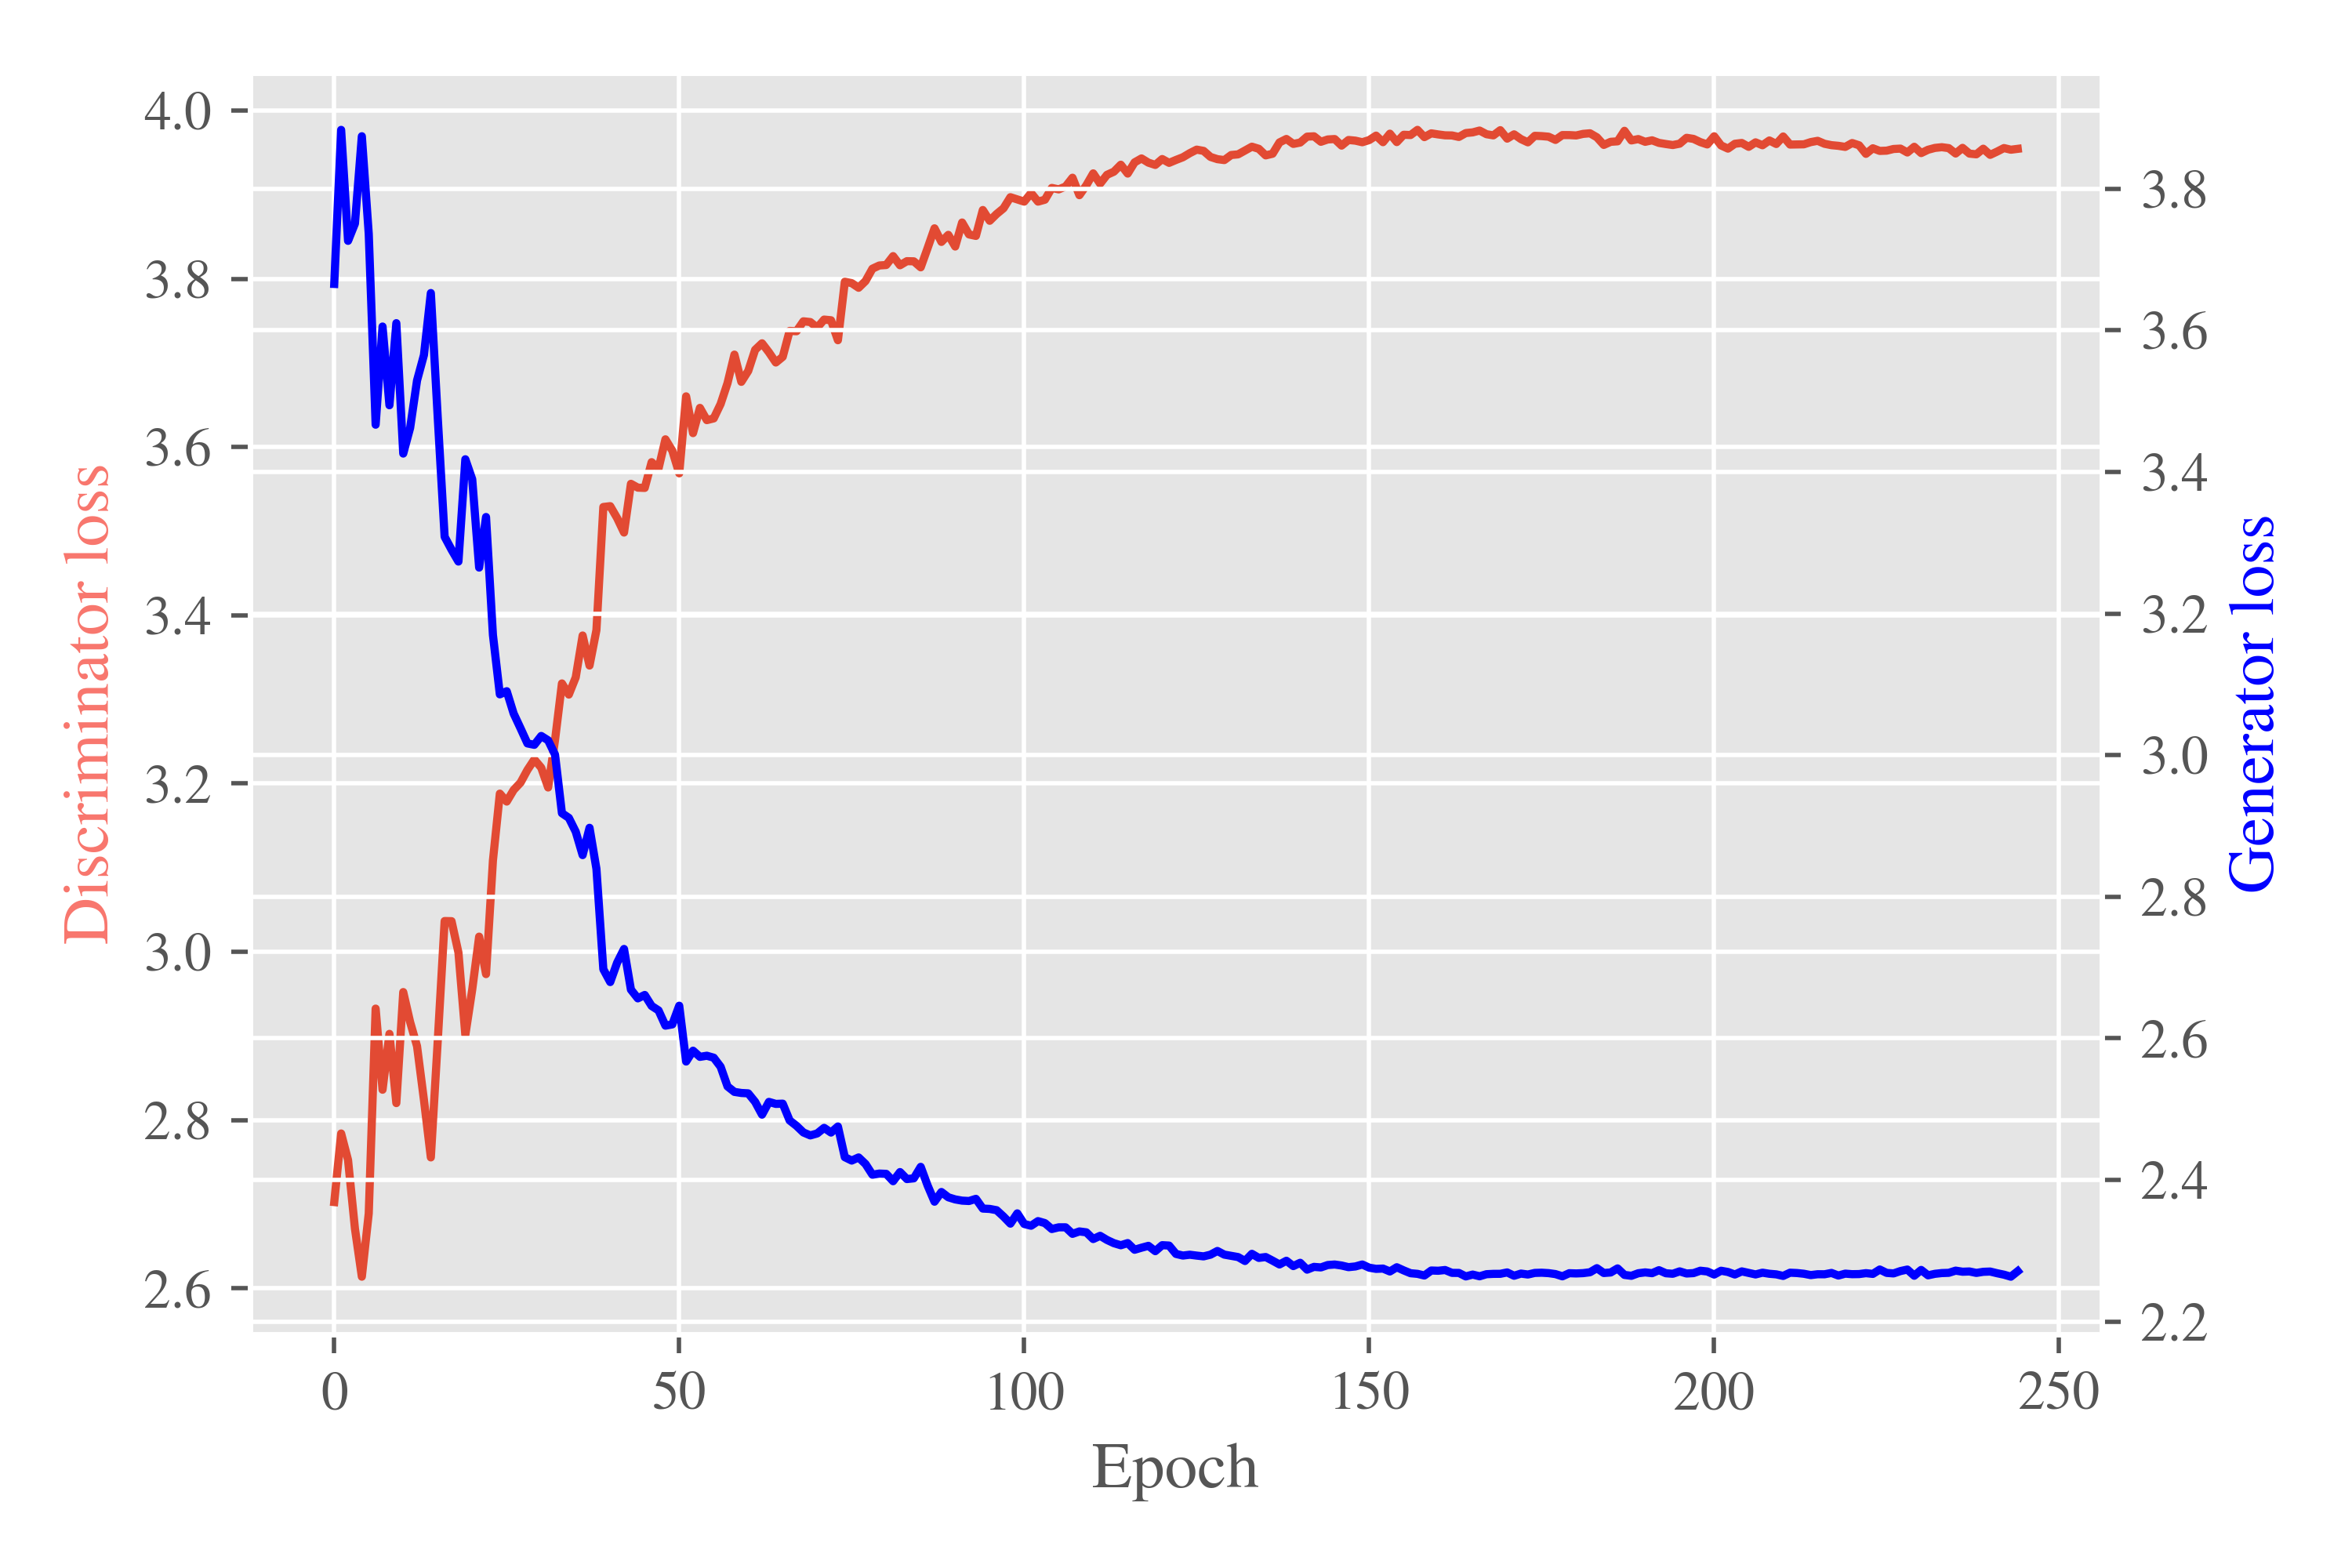
\includegraphics[width=\textwidth]{../code/results/figures/sndcgan_cifar10_losses.png}
		\caption{Losses\\~}
		\label{fig:exp-sndcgan-losses}
    \end{subfigure}
    \caption{SN-DCGAN - training on CIFAR10 over 250 epochs.}
\end{figure}%
We show example generations on both of our datasets:
\begin{figure}[H]
\centering
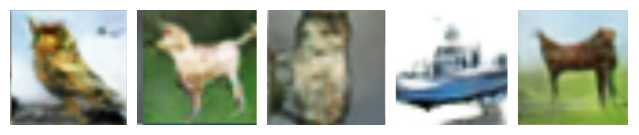
\includegraphics[width=0.7\textwidth]{../code/results/figures/images/sn-dcgan_cifar10}
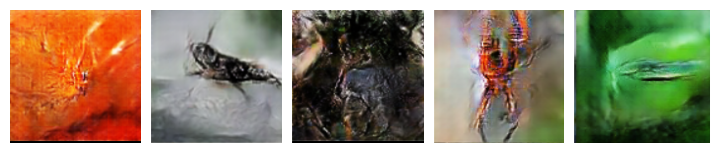
\includegraphics[width=0.7\textwidth]{../code/results/figures/images/sn-dcgan_reptiles}
\caption{SN-DCGAN - generated images after training on CIFAR10 (top) and Reptiles (bottom).}
\end{figure}